\begin{figure}[t]
\centering
\subfigure[\gls{SLIC}]{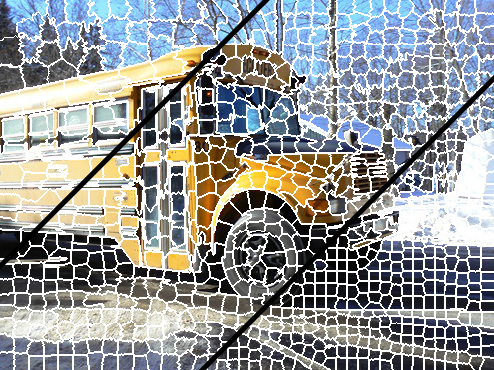
\includegraphics[scale=0.4]{bilder/slic_beispiel}}
\subfigure[Quickshift]{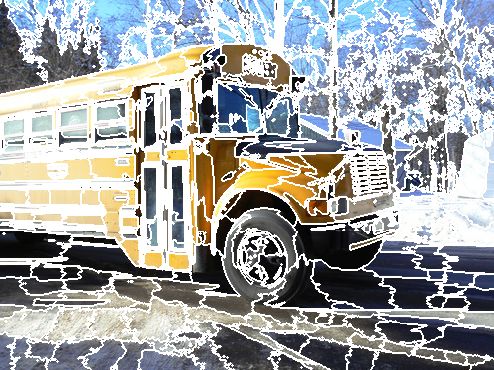
\includegraphics[scale=0.4]{bilder/quickshift_beispiel}}
  \caption[\gls{SLIC} und Quickshift Beispielresultat]{Ein Bus segmentiert über \gls{SLIC} mit jeweils 400, 800 und 1600 Superpixeln (a) sowie über Quickshift mit 600 Superpixeln (b).
  Dabei werden die unterschiedlichen Verfahren zur Generierung von Superpixeln deutlich.
  Wohingegen \gls{SLIC} möglichst quadratische, gleichgroße Superpixel erzeugt, wird die Form der Superpixel von Quickshift größtenteils über die Farbabgrenzungen gesteuert und erzeugt damit sowohl sehr große wie auch sehr kleine Superpixel in allen möglichen Variationen.}
\label{fig:slic_quickshift}
\end{figure}
